\documentclass[class=article, crop=false]{standalone}
\usepackage{tikz}
\usepackage{subcaption}
\usetikzlibrary{calc}
\usetikzlibrary {shapes.geometric}

\begin{document}
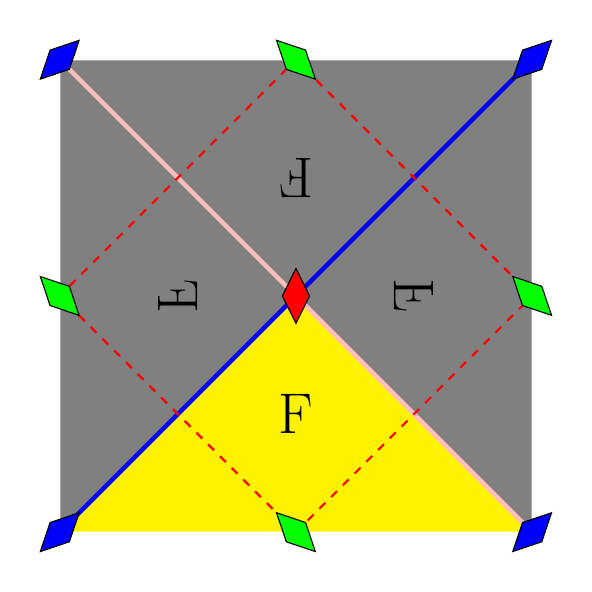
\begin{tikzpicture}
    % Define the lengths of the sides and the angle
    \def\a{3}  % length of side a
    \def\b{3}  % length of side b
    \def\angle{90}  % angle between sides a and b
    \def\s{F} % Label in center of cells

    \def\x{0.4}
    \def\y{0.4}

    % Calculate the coordinates of the points
    \coordinate (C00) at (0, 0);
    \coordinate (C10) at (\a, 0);
    \coordinate (C11) at ({\a + \b*cos(\angle)}, {\b * sin(\angle)});
    \coordinate (C01) at ({\b * cos(\angle)}, {\b * sin(\angle)});
    \coordinate (C02) at ({2*\b*cos(\angle)}, {2*\b * sin(\angle)});
    \coordinate (C12) at ({\a +2*\b * cos(\angle)}, {2*\b * sin(\angle)});
    \coordinate (C22) at ({2*\a + 2*\b * cos(\angle)}, {2*\b * sin(\angle)});
    \coordinate (C21) at ({2*\a + \b*cos(\angle)}, {\b * sin(\angle)});
    \coordinate (C20) at ({2*\a}, 0);

        
    % Draw the oblique unit cell
    \draw[fill=gray,gray] (C00) -- (C20) -- (C22) -- (C02) -- cycle;
    \draw[fill=yellow,yellow] (C00) -- (C11) -- (C20) -- cycle;

    % Draw mirror lines
    \draw[ultra thick,blue] (C00) -- (C22);
    \draw[ultra thick,pink] (C20) -- (C02);
    \draw[thick,dashed,red] (C10) -- (C21) -- (C12) -- (C01) -- cycle;
    
    

    % Draw boundary centre symbols
    %\node[rotate=180] at ($(C00)!0.5!(C01)$) {\huge \s};
    %\node[rotate=0] at ($(C01)!0.5!(C02)$) {\reflectbox{\huge \s}};
    %\node at ($(C20)!0.5!(C21)$) {\huge \s};
    %\node[rotate=180] at ($(C21)!0.5!(C22)$) {\reflectbox{\huge \s}};

    % Create white border
    \draw[fill=white,white] ($(C00)-(\x,\y)$) -- ($(C20)-(-\x,\y)$) -- (C20) -- (C00);
    \draw[fill=white,white] ($(C00)-(\x,-\y)$) -- ($(C02)-(\x,-\y)$) -- (C02) -- (C00);
    \draw[fill=white,white] ($(C02)+(\x,\y)$) -- ($(C22)-(\x,-\y)$) -- (C22) -- (C02);
    \draw[fill=white,white] ($(C20)+(\x,-\y)$) -- ($(C22)+(\x,\y)$) -- (C22) -- (C20);
    
    % Center symbols
    \node at ($(C10)!0.5!(C11)$) {\huge \s};
    \node[rotate=270] at ($(C01)!0.5!(C11)$) {\reflectbox{\huge \s}};
    \node[rotate=180] at ($(C12)!0.5!(C11)$) {\huge \s};
    \node[rotate=90] at ($(C21)!0.5!(C11)$) {\reflectbox{\huge \s}};

    % Draw node rotations
    \draw (C11)  node[rotate = 0,shape aspect=0.5,diamond,draw,fill=red] {};
    \draw (C10)  node[rotate = 45,shape aspect=0.5,diamond,draw,fill=green] {};
    \draw (C01)  node[rotate = 45,shape aspect=0.5,diamond,draw,fill=green] {};
    \draw (C21)  node[rotate = 45,shape aspect=0.5,diamond,draw,fill=green] {};
    \draw (C12)  node[rotate = 45,shape aspect=0.5,diamond,draw,fill=green] {};
    \draw (C00)  node[rotate = 135,shape aspect=0.5,diamond,draw,fill=blue] {};
    \draw (C20)  node[rotate = 135,shape aspect=0.5,diamond,draw,fill=blue] {};
    \draw (C02)  node[rotate = 135,shape aspect=0.5,diamond,draw,fill=blue] {};
    \draw (C22)  node[rotate = 135,shape aspect=0.5,diamond,draw,fill=blue] {};
    
\end{tikzpicture}
\end{document}